\subsubsection{Töpfer's classification} \label{subject_indexing_toepfer}

Töpfer differentiates between lexical and associative indexing approaches and concludes that both approaches complement each other, which is an argument in favor of fusion architectures, the third member of his classification of \acrshort{si} methods \cite{toepfer2020fusion}. We will look at these three groups in this section.

\textit{Associative approaches} find correlations between words \cite{suominen2019annif} by computing co-occurrence statistics, which allow the methods to identify references to the subjects of the \acrshort{kos}. These methods require training data to learn the mappings. Subjects that do not appear in the training data cannot be assigned to any documents, because the model has not learned weights for them. This means that associative approaches require a lot of training data that is well distributed among the subjects, as it is not able to predict unseen subjects.

\textit{Lexical approaches} map salient terms in the document to the subjects using a trained model \cite{suominen2019annif}. KEA++ \cite{medelyan2008domain}, presented in the previous section, is a lexical approach. Because the weights and the threshold are shared by all subjects, lexical models can be used to assign previously unseen subjects. The parameter estimations are reliable because the values computed for each candidate are usually non-vanishing \cite{toepfer2020fusion}. Therefore, not so much training data is required.

Both approaches may lead to low recall. Associative approaches may have low recall when the training data is insufficient. This is likely to be the case because of \textit{Zipf's law}: when ranked by frequency, the frequency of each subject is half of its predecessor. On the other hand, lexical systems may suffer from low recall when the \acrshort{kos} lacks synonyms, which could hamper the hit rate of the string matching step.

\begin{figure}
    \centering
    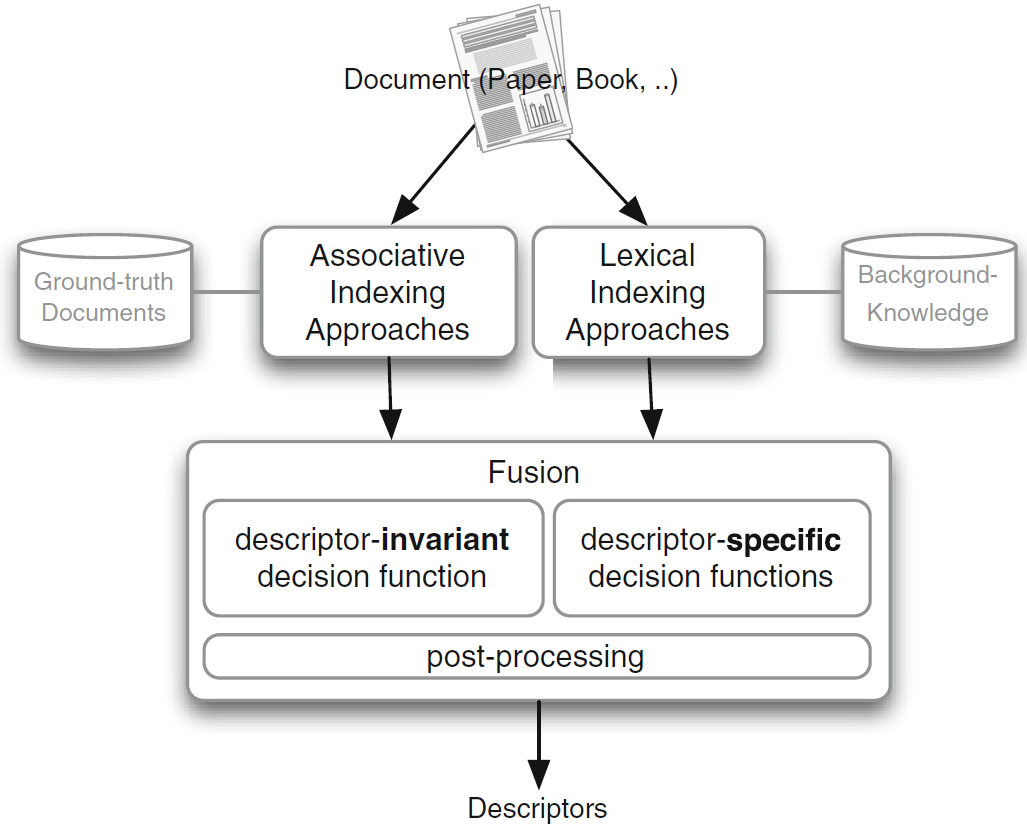
\includegraphics[width=.5\textwidth]{figures/related_work/fusion_architecture.PNG}
    \caption{Schema of a fusion architecture. From \cite{toepfer2020fusion}.}
    \label{fig:fusion_architecture}
\end{figure}

\textit{Fusion architectures} combine lexical and associative indexing systems. Their goal is to gather the advantages of both methods, which were shown to be complementary in the previous section, in one system. Figure \ref{fig:fusion_architecture} shows a schema of the architecture. The decision function, which can be either invariant or specific regarding the subjects, merges the results of the indexing systems into a single set of subjects, which is then assigned to the document after some optional post-processing. The descriptor-invariant decision function may be used for all descriptors, also unseen ones. The descriptor-specific decision function uses the background knowledge and the ground-truth documents to decide on the output.
